
\let\negmedspace\undefined
\let\negthickspace\undefined
\documentclass[journal,12pt,twocolumn]{IEEEtran}

\usepackage{setspace}
\usepackage{gensymb}
\singlespacing
\usepackage[cmex10]{amsmath}

\usepackage{amsthm}

\usepackage{mathrsfs}
\usepackage{txfonts}
\usepackage{stfloats}
\usepackage{bm}
\usepackage{cite}
\usepackage{cases}
\usepackage{subfig}
\usepackage{tabularx}
\usepackage{longtable}
\usepackage{multirow}
\usepackage{tfrupee}
\usepackage{enumitem}
\usepackage{mathtools}
\usepackage{steinmetz}
\usepackage{tikz}
\usepackage{circuitikz}
\usepackage{verbatim}
\usepackage{tfrupee}
\usepackage[breaklinks=true]{hyperref}
\usepackage{graphicx}
\usepackage{tkz-euclide}
\usepackage[utf8]{inputenc}
\usetikzlibrary{calc,math}
\usepackage{listings}
    \usepackage{color}                                            %%
    \usepackage{array}                                            %%
    \usepackage{longtable}                                        %%
    \usepackage{calc}                                             %%
    \usepackage{multirow}                                         %%
    \usepackage{hhline}                                           %%
    \usepackage{ifthen}                                           %%
    \usepackage{lscape}     
\usepackage{multicol}
\usepackage{chngcntr}

\DeclareMathOperator*{\Res}{Res}

\renewcommand\thesection{\arabic{section}}
\renewcommand\thesubsection{\thesection.\arabic{subsection}}
\renewcommand\thesubsubsection{\thesubsection.\arabic{subsubsection}}

\renewcommand\thesectiondis{\arabic{section}}
\renewcommand\thesubsectiondis{\thesectiondis.\arabic{subsection}}
\renewcommand\thesubsubsectiondis{\thesubsectiondis.\arabic{subsubsection}}


\hyphenation{op-tical net-works semi-conduc-tor}
\def\inputGnumericTable{}                                 %%

\lstset{
%language=C,
frame=single, 
breaklines=true,
columns=fullflexible
}
\begin{document}


\newtheorem{theorem}{Theorem}[section]
\newtheorem{problem}{Problem}
\newtheorem{proposition}{Proposition}[section]
\newtheorem{lemma}{Lemma}[section]
\newtheorem{corollary}[theorem]{Corollary}
\newtheorem{example}{Example}[section]
\newtheorem{definition}[problem]{Definition}

\newcommand{\BEQA}{\begin{eqnarray}}
\newcommand{\EEQA}{\end{eqnarray}}
\newcommand{\define}{\stackrel{\triangle}{=}}
\bibliographystyle{IEEEtran}
\raggedbottom
\setlength{\parindent}{0pt}
\providecommand{\mbf}{\mathbf}
\providecommand{\pr}[1]{\ensuremath{\Pr\left(#1\right)}}
\providecommand{\qfunc}[1]{\ensuremath{Q\left(#1\right)}}
\providecommand{\sbrak}[1]{\ensuremath{{}\left[#1\right]}}
\providecommand{\lsbrak}[1]{\ensuremath{{}\left[#1\right.}}
\providecommand{\rsbrak}[1]{\ensuremath{{}\left.#1\right]}}
\providecommand{\brak}[1]{\ensuremath{\left(#1\right)}}
\providecommand{\lbrak}[1]{\ensuremath{\left(#1\right.}}
\providecommand{\rbrak}[1]{\ensuremath{\left.#1\right)}}
\providecommand{\cbrak}[1]{\ensuremath{\left\{#1\right\}}}
\providecommand{\lcbrak}[1]{\ensuremath{\left\{#1\right.}}
\providecommand{\rcbrak}[1]{\ensuremath{\left.#1\right\}}}
\theoremstyle{remark}
\newtheorem{rem}{Remark}
\newcommand{\sgn}{\mathop{\mathrm{sgn}}}
\providecommand{\abs}[1]{\left\vert#1\right\vert}
\providecommand{\res}[1]{\Res\displaylimits_{#1}} 
\providecommand{\norm}[1]{\left\lVert#1\right\rVert}
%\providecommand{\norm}[1]{\lVert#1\rVert}
\providecommand{\mtx}[1]{\mathbf{#1}}
\providecommand{\mean}[1]{E\left[ #1 \right]}
\providecommand{\fourier}{\overset{\mathcal{F}}{ \rightleftharpoons}}
%\providecommand{\hilbert}{\overset{\mathcal{H}}{ \rightleftharpoons}}
\providecommand{\system}{\overset{\mathcal{H}}{ \longleftrightarrow}}
	%\newcommand{\solution}[2]{\textbf{Solution:}{#1}}
\newcommand{\solution}{\noindent \textbf{Solution: }}
\newcommand{\cosec}{\,\text{cosec}\,}
\providecommand{\dec}[2]{\ensuremath{\overset{#1}{\underset{#2}{\gtrless}}}}
\newcommand{\myvec}[1]{\ensuremath{\begin{pmatrix}#1\end{pmatrix}}}
\newcommand{\mydet}[1]{\ensuremath{\begin{vmatrix}#1\end{vmatrix}}}
\numberwithin{equation}{subsection}
\makeatletter
\@addtoreset{figure}{problem}
\makeatother
\let\StandardTheFigure\thefigure
\let\vec\mathbf
\renewcommand{\thefigure}{\theproblem}
\def\putbox#1#2#3{\makebox[0in][l]{\makebox[#1][l]{}\raisebox{\baselineskip}[0in][0in]{\raisebox{#2}[0in][0in]{#3}}}}
     \def\rightbox#1{\makebox[0in][r]{#1}}
     \def\centbox#1{\makebox[0in]{#1}}
     \def\topbox#1{\raisebox{-\baselineskip}[0in][0in]{#1}}
     \def\midbox#1{\raisebox{-0.5\baselineskip}[0in][0in]{#1}}
\vspace{3cm}
\title{CBSE Maths Questions 2019}
\author{Anil Mondedla}
\maketitle
\newpage
\bigskip
\renewcommand{\thefigure}{\theenumi}
\renewcommand{\thetable}{\theenumi}
%
Get latex-tikz codes from 
%
\begin{lstlisting}
https://github.com/AnilMondedla/CBSE
\end{lstlisting}
\section{Section-A}
\begin{enumerate}
\item If in an A.P., a = 15, d = – 3 and $\vec{a}_n = 0$,then find the value of n.\\
\item If sin x + cos y = 1; x = 30\textdegree and y is an acute angle, find the value of y.\\ 
\begin{align}
    \centering \vec{OR}\nonumber
\end{align}
 Find the value of (cos 48\textdegree – sin 42\textdegree).
\item The area of two similar triangles are 25 sq. cm and 121 sq. cm. Find the ratio of their corresponding sides.\\ 

\item The HCF of two numbers a and b is 5 and their LCM is 200. Find the product ab.
\item Find the value of k for which x = 2 is a solution of the equation $ kx^2 + 2x – 3 = 0.$
\begin{align}
    \centering \vec{OR}\nonumber
\end{align}
Find the value/s of k for which the quadratic equation $3x^2 + kx + 3 = 0$ has real and equal roots.

 \item Find the values of x for which the distance between the points A(x, 2) and B(9, 8) is 10 units.
\section{Section-B}
\item A child has a die whose 6 faces show the letters given below :\\
\fbox{A}\;\fbox{B}\;\fbox{C}\;\fbox{A}\;\fbox{A}\;\fbox{B}\\
The die is thrown once. What is the probability of getting (i) A (ii) B ?
\item Find the HCF of 612 and 1314 using prime factorisation.
\begin{align}
    \centering \vec{OR}\nonumber
\end{align}
Show that any positive odd integer is of the form 6m + 1 or 6m + 3 or 6m + 5, where m is some integer.
\item For what value of k, does the system of linear equations 
\begin{align}
   2x + 3y &= 7 \nonumber \\
   (k – 1) x + (k + 2) y &= 3k \nonumber
   \end{align}
have an infinite number of solutions ?
\item If $\vec{S}_n$ , the sum of the first n terms of an A.P. is given by $\vec{S}_n  = 2n^2 + n$, then
find its $n^{\text{th}}$ term.
\begin{align}
    \centering \vec{OR}\nonumber
\end{align}
If the  $17^{\text{th}}$ term of an A.P. exceeds its  $10^{\text{th}}$ term by 7, find the common difference.
\item The mid - point of the line segment joining A(2a, 4) and B(–2, 3b) is (1, 2a + 1). Find the values of a and b.
\item Find the probability that a number selected at random from the numbers 3, 4, 4, 4, 5, 5, 6, 6, 6, 7 will be their mean.
\section{Section-C}
\item In $\vec{\Delta}$ABC, $\angle$ B = 90\textdegree\;and D is the mid-point of BC. Prove that
$AC^2 = AD^2 + 3CD^2$ .
\begin{align}
    \centering \vec{OR}\nonumber
\end{align}
In Figure 1, E is a point on CB produced of an isosceles $\vec{\Delta}$ ABC, with side
AB = AC. If AD $\perp$ BC and EF $\perp$ AC, prove that $\triangle ABD \sim \triangle ECF$.
\begin{figure}[h!]
    \centering
    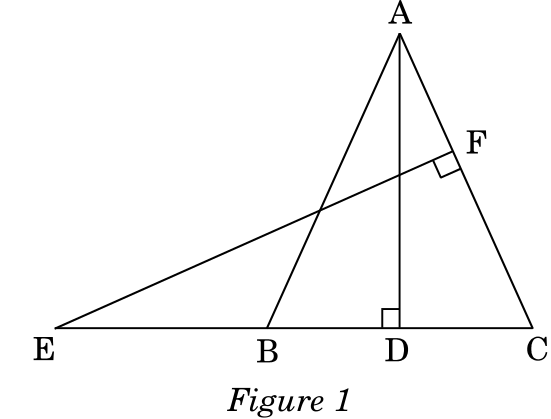
\includegraphics[width=5cm]{1.png}
 \end{figure}
 \item In Figure 2, three sectors of a circle of radius 7 cm, making angles of 60\textdegree,80\textdegree and 40\textdegree at the centre are shaded. Find the the area of the shaded region.
 \begin{figure}[h!]
    \centering
    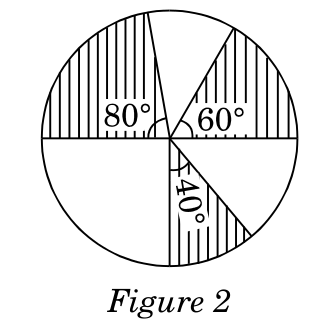
\includegraphics[width=5cm]{2.png}
 \end{figure}
 \item A juice seller was serving his customers using glasses as shown in Figure 3. The inner diameter of the cylindrical glass was 5 cm but bottom of the glass had a hemispherical raised portion which reduced the capacity of the glass. If the height of a glass was 10 cm, find the apparent and actual capacity of the glass. (Use $\pi$ = 3.14)
  \begin{figure}[h!]
    \centering
    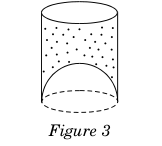
\includegraphics[width=5cm]{3.png}
 \end{figure}
 \begin{align}
    \centering \vec{OR}\nonumber
\end{align}
A girl empties a cylindrical bucket full of sand, of base radius 18 cm and height 32 cm on the floor to form a conical heap of sand. If the height of this conical heap is 24 cm, then find its slant height correct to one place of decimal.
 \medskip
 \item Find all the zeroes of the polynomial $x^4 + x^3 – 14x^2 – 2x + 24$, if two of its zeroes are$\sqrt{2}$  and –$\sqrt{2}$  .
 \medskip
 \item Point P divides the line segment joining the points A(2, 1) and B(5, –8) such that
 $ \displaystyle\frac{AP}{AB}=\displaystyle\frac{1}{3}$ If P lies on the line $2x – y + k = 0$, find the value of k.
  \begin{align}
    \centering \vec{OR}\nonumber
\end{align}
For what value of p, are the points (2, 1), (p,–1) and (–1, 3) collinear ?\\
\item Prove that :
\begin{center}
 $ \displaystyle\frac{\tan\theta}{1 – \tan\theta} - \displaystyle\frac{\cot\theta}{1 – \cot\theta} = \displaystyle\frac{\cos\theta+\sin\theta}{\cos\theta - \sin\theta}$
\end{center}
  \begin{align}
    \centering \vec{OR}\nonumber
\end{align}
If $\cos\theta + \sin\theta=\sqrt{2} \cos\theta$, show that $\cos\theta – \sin\theta = \sqrt{2}\sin\theta$
 \medskip
\item A part of monthly hostel charges in a college hostel are fixed and the remaining depends on the number of days one has taken food in the mess. When a student A takes food for 25 days, he has to pay \rupee~4,500, whereas a student B who takes food for 30 days, has to pay \rupee~5,200. Find the fixed charges per month and the cost of food per day.\\
\item Find the mode of the following frequency distribution :
	\begin{table}[hbt]
\centering
	\resizebox{\columnwidth}{!}{
\begin{tabular}{ |c|c|c|c|c|c|c|c| } 
\hline
{Class :}&10-14&14–18&18–22&22–26&26–30&30–34&34–38\\
\hline
{Frequency :}&8&6&11&20&25&22&10\\ 
\hline
\end{tabular}
}
\end{table}
\\
 \item In two concentric circles, prove that all chords of the outer circle which touch the inner circle, are of equal length.
 \medskip
 \item Prove that $(5 – 3\sqrt{2})$ is an irrational number, given that $\sqrt{2}$ is irrational number.
 \bigskip
 \section{Section-D}
 \item A boy standing on a horizontal plane finds a bird flying at a distance of 100 m from him at an elevation of 30\textdegree. A girl standing on the roof of a 20 m high building, finds the elevation of the same bird to be 45\textdegree. The boy and the girl are on the opposite sides of the bird. Find the distance of the
bird from the girl.(Given $\sqrt{2} = 1·414$)
\begin{align}
    \centering \vec{OR}\nonumber
\end{align}
The angle of elevation of an aeroplane from a point A on the ground is $60\textdegree$. After a flight of 30 seconds, the angle of elevation changes to 30\textdegree. If the plane is flying at a constant height of 3600$\sqrt{3}$ metres, find the speed of the aeroplane.\\
\bigskip
\item Find the values of frequencies x and y in the following frequency distribution table, if N = 100 and median is 32.
\begin{table} [htb]
\centering
\resizebox{\columnwidth}{!}{
\begin{tabular}{ |c|c|c|c|c|c|c|c|c| } 
\hline
{Marks :}& 0 - 10 &10 - 20 & 20 - 30&30 - 40 &40 - 50&50 - 60&Total\\
\hline
{No. of Students :}& 10 & x & 25& 30&y&10&100\\ 
\hline
\end{tabular}
}
\end{table}
\begin{align}
    \centering \vec{OR}\nonumber
\end{align}
For the following frequency distribution, draw a cumulative frequency curve (ogive) of ‘more than type’ and hence obtain the median value.\\
\begin{table}[htb]
	\centering
	\resizebox{\columnwidth}{!}{
\begin{tabular}{ |c|c|c|c|c|c|c|c| } 
\hline
{Class :}& 0 – 10 &10 – 20 & 20 – 30&30 – 40 &40 – 50&50 – 60&60-70\\
\hline
{Frequency :}& 5 & 15 & 20& 23&17&11&9\\ 
\hline
\end{tabular}
}
\end{table}
\item  Prove that :
\begin{center}
 $\displaystyle\frac{(1+\cot\theta+\tan\theta)(\sin\theta-\cos\theta)}{\sec^3\theta-\cosec^3\theta} = \sin^2\theta\; \cos^2\theta$
\end{center}
\item  An open metallic bucket is in the shape of a frustum of a cone. If the diameters of the two circular ends of the bucket are 45 cm and 25 cm and the vertical height of the bucket is 24 cm, find the area of the metallic sheet used to make the bucket. Also find the volume of the water it can hold.(Use $\pi$= $\frac{22}{7}$)
\medskip
\item A train travels 360 km at a uniform speed. If the speed had been 5 km/hr
more, it would have taken 1 hr less for the same journey. Find the speed
of the train.
 \begin{align}
    \centering \vec{OR}\nonumber
\end{align}
Solve for x :
\begin{center}
	$\displaystyle\frac{1}{a+b+x}= \frac{1}{a}+\frac{1}{b}+\frac{1}{x};a\neq b \neq 0,x \neq 0 ,
x\neq -(a+b)$
\end{center}
\item In an AP.,the $n^{\text{th}}$ term is $\displaystyle\frac{1}{m}$ and the $m^{\text{th}}$ term is $\displaystyle\frac{1}{n}$ Find (i) $(mn)^{\text{th}}$ term, (ii) sum of first (mn) terms.
\item Prove that in a right triangle, the square of the hypotenuse is equal to
the sum of the squares of the other two sides.
\medskip
\item Construct a pair of tangents to a circle of radius 4 cm which are inclined
to each other at an angle of 60\textdegree.\\

 \end{enumerate}
\end{document}
